\documentclass[12pt]{article}
\usepackage[letterpaper, margin=0.8in]{geometry}
\usepackage{nopageno,epsfig, amsmath, amssymb}
\usepackage{physics}
\usepackage{mathtools}
\usepackage{hyperref}
\usepackage{xcolor}
\usepackage{natbib}
\hypersetup{
    colorlinks,
    linkcolor={blue},
    citecolor={blue},
    urlcolor={blue}
}
\usepackage{empheq}
\usepackage{wrapfig}

\usepackage{fancyhdr, titling}

\usepackage{parskip}
\setlength{\parindent}{0pt}

\usepackage{../aas_macros}

\title{Physics of Period Spacing Patterns}
\author{\textbf{Tom Wagg}}

\pagestyle{fancy}
\fancyhf{}
\rhead{\theauthor}
\lhead{\thetitle}
\rfoot{Page \thepage}

\newcommand{\tomtitle}{
    \noindent {\LARGE \fontfamily{cmr}\selectfont \textbf{\thetitle}} \hfill \\[1\baselineskip]
    \noindent {\large \fontfamily{cmr}\selectfont Kavli Summer Program \hfill \textsc{Tom Wagg}}\\[0.5\baselineskip]
}

\newcommand{\question}[1]{{\noindent \it #1}}
\newcommand{\answer}[1]{
    \par\noindent\rule{\textwidth}{0.4pt}#1\vspace{0.5cm}
}
\newcommand{\todo}[1]{{\color{red}\begin{center}TODO: #1\end{center}}}

% custom function for adding units
\makeatletter
\newcommand{\unit}[1]{%
    \,\mathrm{#1}\checknextarg}
\newcommand{\checknextarg}{\@ifnextchar\bgroup{\gobblenextarg}{}}
\newcommand{\gobblenextarg}[1]{\,\mathrm{#1}\@ifnextchar\bgroup{\gobblenextarg}{}}
\makeatother

\newcommand{\avg}[1]{\left\langle #1 \right\rangle}
\newcommand{\angstrom}{\mbox{\normalfont\AA}}
\allowdisplaybreaks

\begin{document}

\tomtitle{}

\thispagestyle{empty}

Here are some notes to ensure I actually understand what I'm talking about :D

Let's start with an equation, because that's how my brain works. I think this is called the asymptotic approximation. Anyway under the assumption of spherical symmetry (we're ignoring rotation folks) and high-order: the g-mode period spacing (i.e. the difference in period between modes of the same spherical degree and neighbouring radial order) is approximately constant and given by \citep[e.g.,][]{Hatta+2023}
\begin{equation}
    \Delta P_g = \frac{\pi^2}{\sqrt{l(l+1)}} \qty[\int_{r_0}^{r_1} \frac{N}{r} \dd{r}]^{-1},
\end{equation}
where $l$ is the spherical degree and
\begin{equation}
    N^2 \approxeq \frac{g^2 \rho}{P} \qty(\grad_{\rm ad} - \grad + \grad_\mu),
\end{equation}
is the Brunt Vaisala (BV) frequency which is integrated within the g-mode cavity. Recall that $\grad_{\rm ad}$ is a constant (equal to 2/5 for an ideal gas), $\grad$ is the temperature gradient and $\grad_\mu$ is the chemical composition gradient.

This means that the period spacing, for a fixed spherical degree, is dependent on the location of
\begin{enumerate}
    \item The core boundary (I'm assuming the cavity extends to the edge of the star so $r_1$ is fixed)
    \item The BV frequency profile
\end{enumerate}
For more massive stars, the size of the convective core increases, which reduces the size of the g-mode cavity and thus decreases the integral. This tends to dominate over any changes in the BV profile and so the overall period spacing increases almost monotonically along with stellar evolution \citep{Miglio+2008}.

In addition to these effects, we haven't even thought about rotation yet! This is a rather glaring omission since we expect some pretty fast rotation for our target stars it seems. Under the traditional approximation of rotation (TAR), the period spacing is quasi-linearly related to period rather than constant, and the rate of this rotation determines the gradient of the relation \citep{Bouabid+2013}. So essentially instead of a flat line we expect increasingly slanted lines for faster rotating stars. I \textit{think} that Cole also mentioned that the gradient of this line will flip for retrograde rotators.

So what happens when we get deviations from our beautiful straight lines, what's up with that? These occur due to abrupt shifts in the BV profile, sometimes referred to as buoyancy glitches \citep[e.g.,][]{Cunha+2019}, which end up trapping particular modes in certain regions of the star. This means that certain modes end up getting shifted in period and moving away from the pattern.

Okay well why do those glitches in the BV profile happen? Often strong chemical gradients cause these effects and we can see this in general around the boundary of the convective core where the chemical composition changes rapidly. In Figure~\ref{fig:prop} you can see an example propagation diagram for a $4 \unit{M_{\odot}}$ star midway through its main sequence. The purple curve shows the BV profile and in particular a sharp feature around $1 \unit{M_{\odot}}$, corresponding to the boundary of the convective core.
\begin{figure}[htb]
    \centering
    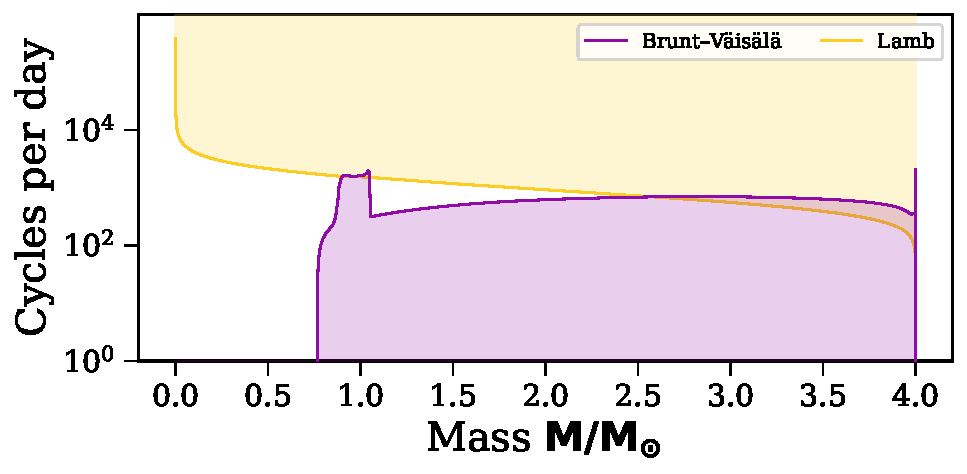
\includegraphics[width=0.75\textwidth]{example_propagation_diagram.pdf}
    \caption{An example propagation diagram for a $4 \protect\unit{M_{\odot}}$ star midway through its main sequence.}
    \label{fig:prop}
\end{figure}

These same sharp features should occur after a star experiences mass transfer and so we might expect that the period spacing pattern bears some imprint of the stars previous mass transfer episode - we've got 4 more weeks to find out if that's true and how it might look!

\bibliographystyle{aasjournal}
\bibliography{refs}

\end{document}

 